\subsection{Problem}
\renewcommand{\theequation}{\theenumi}
\begin{enumerate}[label=\thesection.\arabic*.,ref=\thesection.\theenumi]
\numberwithin{equation}{enumi}
	\item Find all pairs of consecutive odd natural numbers, both of which are greater than 10, such that their sum is less than 40.\\
	The following python code computes the required pairs of consecutive odd natural numbers which satisfy the required condition, shown in Fig.\ref{fig:qfifteen}.
	\begin{lstlisting}
	./codes/lines/q15.py
	\end{lstlisting}
	
	\solution Let x be an odd natural number and y be the odd natural number consecutive to x.
	\begin{align}
	\therefore y=x+2
	\end{align}
	We need to find x and y  such that 
	\begin{multline}
x,y >10 \text{ and } x+y<40\\
\therefore x+x+2<40\\
2x+2<40\\
x+1<20\\
x<19\\
	\end{multline}
	
	
	Hence the condition is satisfied when $x>10$ and $x<19$
	
	\begin{figure}[!ht]
	\centering
	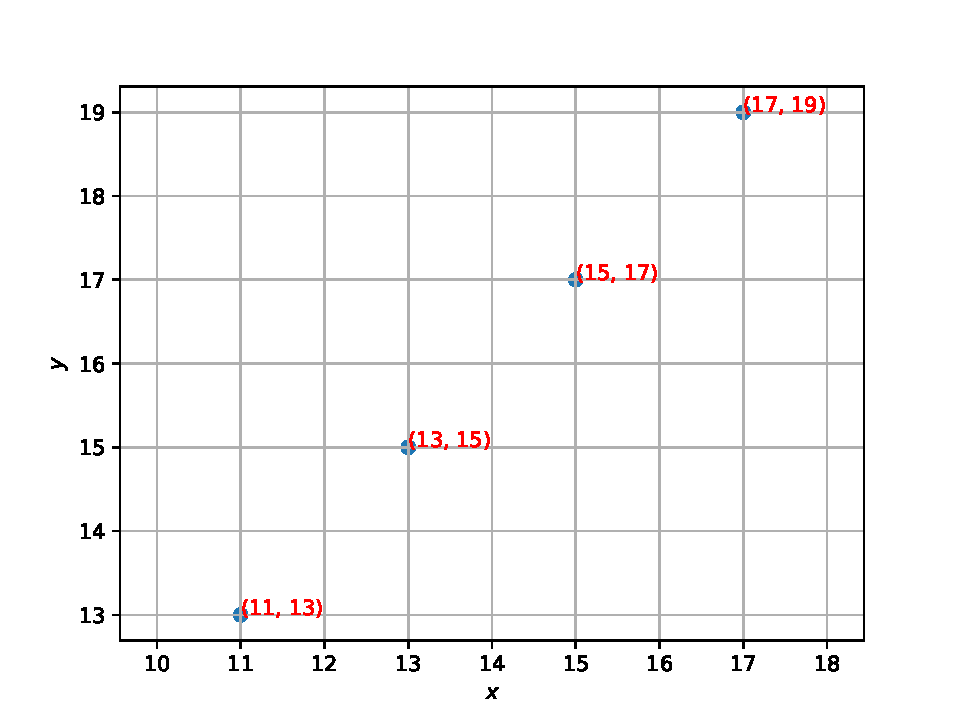
\includegraphics[width=\columnwidth]{./figs/lines/q15.pdf}
	\caption{Triangle of Q.3.11.5}
	\label{fig:qfifteen}	
	\end{figure}
	
	
\end{enumerate}
